% Fig 2: NeuroPLC Compiler Architecture
% Compile: xelatex fig2_compiler_arch.tex
\documentclass[tikz,border=8pt]{standalone}
\usepackage{tikz}
\usepackage{fontspec}
\usetikzlibrary{shapes.geometric, arrows.meta, positioning, calc, fit, backgrounds, shadows}

\definecolor{steel}{HTML}{2563eb}
\definecolor{teal}{HTML}{0d9488}
\definecolor{amber}{HTML}{d97706}
\definecolor{slate}{HTML}{64748b}
\definecolor{rose}{HTML}{e11d48}
\definecolor{ink}{HTML}{1e293b}
\definecolor{snow}{HTML}{fafbfc}
\definecolor{purple}{HTML}{7c3aed}
\definecolor{cyan}{HTML}{06b6d4}

\begin{document}
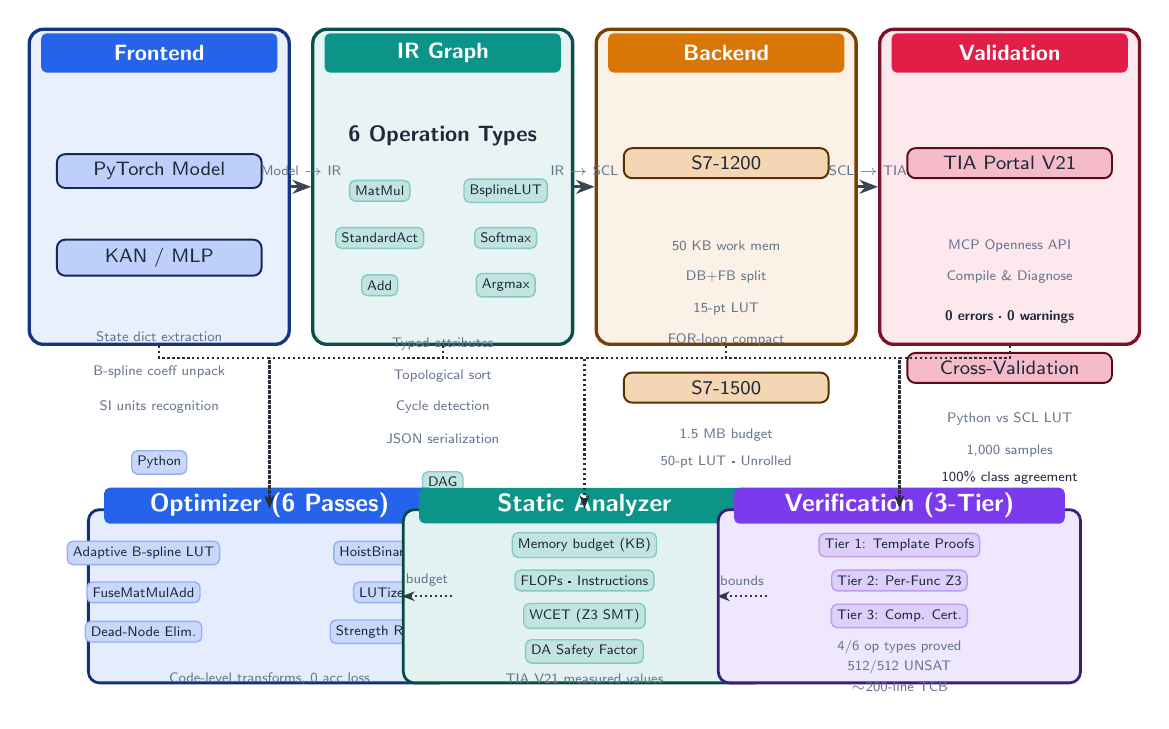
\begin{tikzpicture}[
    % ── Main stage container ──
    mainbox/.style={
        rectangle, rounded corners=5pt,
        draw=#1!55!black, fill=#1!10, line width=1.2pt,
        text=ink, minimum width=3.3cm, minimum height=4.0cm,
        font=\sffamily, align=center, inner sep=4pt,
    },
    % ── Title bar ──
    titler/.style={
        rectangle, rounded corners=2pt,
        fill=#1, text=white,
        font=\sffamily\footnotesize\bfseries, align=center,
        minimum width=3.0cm, minimum height=0.5cm, inner sep=2pt,
    },
    % ── Sub-box inside main section ──
    subbox/.style={
        rectangle, rounded corners=3pt,
        draw=#1!40!black, fill=#1!30, line width=0.7pt,
        text=ink, font=\sffamily\scriptsize, align=center,
        inner sep=3pt, minimum width=2.6cm,
    },
    % ── Bottom panel ──
    panel/.style={
        rectangle, rounded corners=4pt,
        draw=#1!50!black, fill=#1!12, line width=1.0pt,
        text=ink, minimum width=4.6cm, minimum height=2.2cm,
        font=\sffamily\footnotesize, align=center, inner sep=5pt,
    },
    % ── Panel title ──
    ptitle/.style={
        rectangle, rounded corners=2pt,
        fill=#1, text=white,
        font=\sffamily\small\bfseries, align=center,
        minimum width=4.2cm, minimum height=0.45cm, inner sep=2pt,
    },
    % ── Arrows ──
    arr/.style={
        -{Stealth[scale=0.8]}, line width=1.2pt, slate!60!black,
    },
    arrlight/.style={
        -{Stealth[scale=0.7]}, line width=0.8pt, slate!40!black,
        densely dotted,
    },
    % ── Small tag badges ──
    tag/.style={
        rectangle, rounded corners=2pt, fill=#1!25,
        draw=#1!50, line width=0.5pt,
        font=\sffamily\tiny, text=ink, inner sep=2pt,
    },
]

% ============================================================
% TOP ROW: 4 Main Pipeline Stages
% ============================================================
% x positions: -5.4, -1.8, 1.8, 5.4  (spaced 3.6cm apart)

% ── S1: FRONTEND ──
\node[mainbox=steel] (FE) at (-5.4, 2.0) {};
\node[titler=steel] at (-5.4, 3.7) {Frontend};
\node[subbox=steel] at (-5.4, 2.2) {PyTorch Model};
\node[subbox=steel] at (-5.4, 1.1) {KAN / MLP};
\node[font=\sffamily\tiny, text=slate] at (-5.4, 0.1) {State dict extraction};
\node[font=\sffamily\tiny, text=slate] at (-5.4, -0.35) {B-spline coeff unpack};
\node[font=\sffamily\tiny, text=slate] at (-5.4, -0.8) {SI units recognition};
\node[tag=steel] at (-5.4, -1.5) {Python};

% ── S2: IR GRAPH ──
\node[mainbox=teal] (IR) at (-1.8, 2.0) {};
\node[titler=teal] at (-1.8, 3.7) {IR Graph};
\node[font=\sffamily\footnotesize\bfseries, text=ink] at (-1.8, 2.65) {6 Operation Types};
% Op type tags
\node[tag=teal] at (-2.6, 1.95) {MatMul};
\node[tag=teal] at (-1.0, 1.95) {BsplineLUT};
\node[tag=teal] at (-2.6, 1.35) {StandardAct};
\node[tag=teal] at (-1.0, 1.35) {Softmax};
\node[tag=teal] at (-2.6, 0.75) {Add};
\node[tag=teal] at (-1.0, 0.75) {Argmax};
% Annotation
\node[font=\sffamily\tiny, text=slate] at (-1.8, 0.0) {Typed attributes};
\node[font=\sffamily\tiny, text=slate] at (-1.8, -0.4) {Topological sort};
\node[font=\sffamily\tiny, text=slate] at (-1.8, -0.8) {Cycle detection};
\node[font=\sffamily\tiny, text=slate] at (-1.8, -1.2) {JSON serialization};
\node[tag=teal] at (-1.8, -1.75) {DAG};

% ── S3: BACKEND ──
\node[mainbox=amber] (BE) at (1.8, 2.0) {};
\node[titler=amber] at (1.8, 3.7) {Backend};
\node[subbox=amber] at (1.8, 2.3) {S7-1200};
\node[font=\sffamily\tiny, text=slate] at (1.8, 1.25) {50 KB work mem};
\node[font=\sffamily\tiny, text=slate] at (1.8, 0.85) {DB+FB split};
\node[font=\sffamily\tiny, text=slate] at (1.8, 0.45) {15-pt LUT};
\node[font=\sffamily\tiny, text=slate] at (1.8, 0.05) {FOR-loop compact};
\node[subbox=amber] at (1.8, -0.55) {S7-1500};
\node[font=\sffamily\tiny, text=slate] at (1.8, -1.15) {1.5 MB budget};
\node[font=\sffamily\tiny, text=slate] at (1.8, -1.5) {50-pt LUT · Unrolled};
\node[tag=amber] at (1.8, -2.05) {IEC 61131-3 SCL};

% ── S4: VALIDATION ──
\node[mainbox=rose] (VAL) at (5.4, 2.0) {};
\node[titler=rose] at (5.4, 3.7) {Validation};
\node[subbox=rose] at (5.4, 2.3) {TIA Portal V21};
\node[font=\sffamily\tiny, text=slate] at (5.4, 1.25) {MCP Openness API};
\node[font=\sffamily\tiny, text=slate] at (5.4, 0.85) {Compile \& Diagnose};
\node[font=\sffamily\tiny, text=ink] at (5.4, 0.35) {\textbf{0 errors · 0 warnings}};
\node[subbox=rose] at (5.4, -0.3) {Cross-Validation};
\node[font=\sffamily\tiny, text=slate] at (5.4, -0.95) {Python vs SCL LUT};
\node[font=\sffamily\tiny, text=slate] at (5.4, -1.35) {1,000 samples};
\node[font=\sffamily\tiny, text=ink] at (5.4, -1.7) {100\% class agreement};
\node[tag=rose] at (5.4, -2.25) {S7-1200|1500};

% ── Arrows: main pipeline ──
\draw[arr] (FE.east) -- (IR.west) node[midway, above, font=\sffamily\tiny, text=slate] {Model $\to$ IR};
\draw[arr] (IR.east) -- (BE.west) node[midway, above, font=\sffamily\tiny, text=slate] {IR $\to$ SCL};
\draw[arr] (BE.east) -- (VAL.west) node[midway, above, font=\sffamily\tiny, text=slate] {SCL $\to$ TIA};

% ============================================================
% BOTTOM ROW: 3 Panels (cross-cutting)
% ============================================================
% x positions: -4.0, 0.0, 4.0

% ── Panel 1: OPTIMIZER ──
\node[panel=steel] (OPT) at (-4.0, -3.2) {};
\node[ptitle=steel] at (-4.0, -2.05) {Optimizer (6 Passes)};
% Passes as tags
\node[tag=steel] at (-5.6, -2.65) {Adaptive B-spline LUT};
\node[tag=steel] at (-5.6, -3.15) {FuseMatMulAdd};
\node[tag=steel] at (-2.4, -2.65) {HoistBinarySearch};
\node[tag=steel] at (-2.4, -3.15) {LUTizeEXP};
\node[tag=steel] at (-5.6, -3.65) {Dead-Node Elim.};
\node[tag=steel] at (-2.4, -3.65) {Strength Reduction};
\node[font=\sffamily\tiny, text=slate] at (-4.0, -4.25) {Code-level transforms, 0 acc loss};

% ── Panel 2: STATIC ANALYZER ──
\node[panel=teal] (ANL) at (0.0, -3.2) {};
\node[ptitle=teal] at (0.0, -2.05) {Static Analyzer};
\node[tag=teal] at (0.0, -2.55) {Memory budget (KB)};
\node[tag=teal] at (0.0, -3.0) {FLOPs · Instructions};
\node[tag=teal] at (0.0, -3.45) {WCET (Z3 SMT)};
\node[tag=teal] at (0.0, -3.9) {DA Safety Factor};
\node[font=\sffamily\tiny, text=slate] at (0.0, -4.25) {TIA V21 measured values};

% ── Panel 3: VERIFICATION ──
\node[panel=purple] (VFY) at (4.0, -3.2) {};
\node[ptitle=purple] at (4.0, -2.05) {Verification (3-Tier)};
\node[tag=purple] at (4.0, -2.55) {Tier 1: Template Proofs};
\node[tag=purple] at (4.0, -3.0) {Tier 2: Per-Func Z3};
\node[tag=purple] at (4.0, -3.45) {Tier 3: Comp. Cert.};
\node[font=\sffamily\tiny, text=slate] at (4.0, -3.85) {4/6 op types proved};
\node[font=\sffamily\tiny, text=slate] at (4.0, -4.1) {512/512 UNSAT};
\node[font=\sffamily\tiny, text=slate] at (4.0, -4.35) {$\sim$200-line TCB};

% ── Arrows: main boxes to panels ──
\draw[arrlight] (FE.south) -- ++(0,-0.15) -| (OPT.north);
\draw[arrlight] (IR.south) -- ++(0,-0.15) -| (OPT.north);
\draw[arrlight] (IR.south) -- ++(0,-0.15) -| (ANL.north);
\draw[arrlight] (BE.south) -- ++(0,-0.15) -| (ANL.north);
\draw[arrlight] (BE.south) -- ++(0,-0.15) -| (VFY.north);
\draw[arrlight] (VAL.south) -- ++(0,-0.15) -| (VFY.north);

% ── Loop arrows among panels ──
\draw[arrlight, slate!50!black] (OPT.east) -- (ANL.west)
    node[midway, above, font=\sffamily\tiny, text=slate] {budget};
\draw[arrlight, slate!50!black] (ANL.east) -- (VFY.west)
    node[midway, above, font=\sffamily\tiny, text=slate] {bounds};

\end{tikzpicture}
\end{document}
